\documentclass[11pt]{article}

\usepackage[
%	top=20mm,
%	bottom=20mm,
%	left=20mm,
%	right=20mm,
%	includehead
a4paper,
%scale={0.8,0.5},
%includeheadfoot,
includefoot,
ignoremp,
%ignorefoot,
layouthoffset=0pt,
top=3.5cm,
bottom=1.25cm,
footskip=1.25cm,
headsep=2cm,
scale=0.7,ignorehead,
headheight=21pt
%showframe
]{geometry}
\usepackage{array}
\usepackage{graphicx}
\usepackage{color}

%\includegraphics[height=3cm]{example-image.pdf}%

\usepackage{testpackage}
\usepackage{pgfplots}
\setromanfont{Fira Sans}
\setmainfont{Fira Sans}
\everymath\expandafter{\the\everymath\rm}
\everydisplay\expandafter{\the\everydisplay\rm}
\pagestyle{fancy}
\fancyheadoffset[]{50pt}
\lhead{\rule{\linewidth}{2pt}\\ \hspace{1cm} }
% \lhead{Δημήτρης Τσορτανίδης}
\chead{ΔΗΜΗΤΡΗΣ ΤΣΟΡΤΑΝΙΔΗΣ ΜΑΘΗΜΑΤΙΚΟΣ MSc}
\rhead{2018}
%\setlength{\textwidth}{0.6\paperwidth} 

\usepackage{xgreek}
\usepackage{setspace}
\usepackage{pdfpages}
\renewcommand{\baselinestretch}{1.5} 
\usepackage{multicol}% \setlength{\columnsep}{1cm}
\usepackage[export]{adjustbox}%Βάζει το πάνω μέρος της εικόνας στην αρχή της λίστας
%%%%%%%%%%%%%%%%%%%%%%%%%%
%\usepackage{showframe}
%%%%%%%%%%%%%%%%%%%%%%%%%
\usepackage{endnotes}
					\renewcommand{\makeenmark}{\textbf{\theenmark. }}
					\renewcommand{\notesname}{Απαντήσεις \hrule}
					\newcommand{\solution}[1]{\endnotetext[\value{enumi}]{#1}}
\begin{document}

\begin{center}
\huge{ΕΦΑΡΜΟΓΗ ΣΤΑ ΠΟΛΥΩΝΥΜΑ}

\end{center}
\rule{\textwidth}{2pt}

\section*{Εισαγωγή}
Το Κεφάλαιο 3 της Άλγεβρας Β Λυκείου ασχολείται με τα πολυώνυμα. Γίνεται μελέτη των χαρακτηριστικών τους και παρουσιάζονται θεωρήματα τα οποία καλύπτουν έννοιες όπως η διαίρεση των πολυωνύμων, η επίλυση εξισώσεων και ανισώσεων κ.α.. Προκύπτει όμως το ερώτημα:
\begin{center}

	\textbf{"Γιατί η μελέτη των πολυωνύμων είναι σημαντική;"}.
\end{center}

Πέρα από τη χρησιμοθηρική προσέγγιση που αφορά τη συχνή τους χρήση στην επίλυση προβλημάτων στα πλαίσια του σχολείου και των Πανελλαδικών Εξετάσεων, θα παρουσιάσουμε μία εφαρμογή χρήσης των πολυωνύμων για την προσέγγιση άλλων περισσότερο "δύσκολων συναρτήσεων."
\setlength{\columnsep}{20pt}\setlength{\columnseprule}{0pt}
\section*{Προσέγγιση του συνημιτόνου}
\begin{multicols}{2}
Στο Κεφάλαιο 2 της Άλγεβρας συναντήσαμε την τριγωνομετρική συνάρτηση ${f(x)=συνx}$, την οποία μελετήσαμε ως προς την περίοδό της, τη μονοτονία της και τελικά με τη γραφική της παράσταση. Όποτε χρειάστηκε ο υπολογισμός της τιμής του συνημιτόνου μίας γωνίας, χρησιμοποιήθηκε είτε ο διαθέσιμος πίνακας τριγωνομετρικών αριθμών, ο οποίος βέβαια αναφέρεται στους τριγωνομετρικούς αριθμούς συγκεκριμένων γνωστών γωνιών, είτε χρησιμοποιήσαμε τις γνωστές τριγωνομετρικές ταυτότητες για το υπολογισμό ενός τριγωνομετρικού αριθμού εφόσον γνωρίζαμε κάποιον άλλο. Για παράδειγμα ο υπολογισμός των τριγωνομετρικών αριθμών της γωνίας $\dfrac{π}{16}$ από τους τριγωνομετρικούς αριθμούς της γνωστής γωνίας $\dfrac{π}{4}$ και τη χρήση των τριγωνομετρικών ταυτοτήτων των $ημ2α$,$συν2α$.

Παρόλα αυτά υπάρχει τρόπος χρησιμοποιώντας γνωστό θεώρημα να προσδιορίσουμε τους συντελεστές ενός πολυωνύμου, οι τιμές του οποίου θα βρίσκονται πολύ κοντά στην τιμή του αντίστοιχου τριγωνομετρικού αριθμού. Όπως φαίνεται και στην εικόνα που ακολουθεί, όσο μεγαλύτερος είναι ο βαθμός του πολυωνύμου, τόσο πιο "κοντά" στη συνάρτηση που θέλουμε να προσεγγίσουμε. Με τον τρόπο αυτό ο υπολογισμός της τιμής του συνημιτόνου μιας γωνίας για παράδειγμα ανάγεται στον πολύ ευκολότερο υπολογισμό της τιμής ενός πολυωνύμου. 
\end{multicols}
Παρακάτω φαίνεται η προσέγγιση της συνάρτησης $συνx$ με το πολυώνυμο \[P(x)=1-\dfrac{x^2}{2!}+\dfrac{x^4}{4!}-\dfrac{x^6}{6!}\dotsc\]
όπου $ν!=1\cdot2\cdot3\cdot4\dots ν$\setlength{\columnsep}{10pt}\setlength{\columnseprule}{0pt}
\begin{center}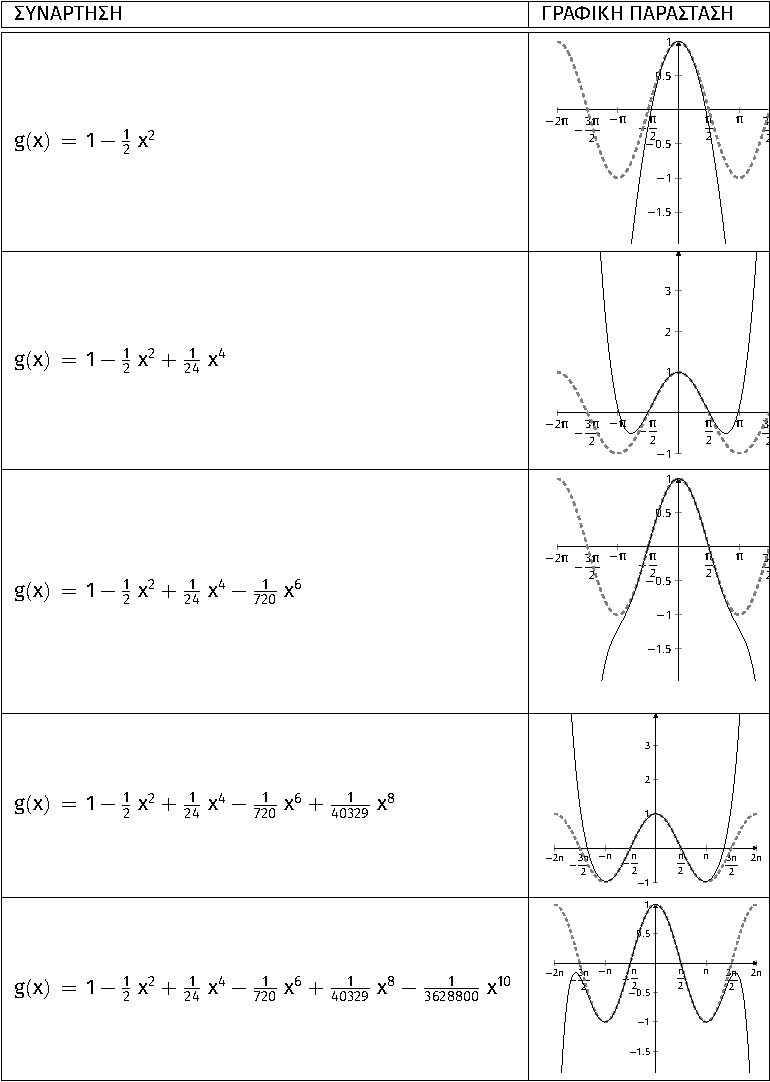
\includegraphics[width=0.8\textwidth]{tikzpic1.pdf}\end{center}
%\begin{figure}[h]
%	\centering	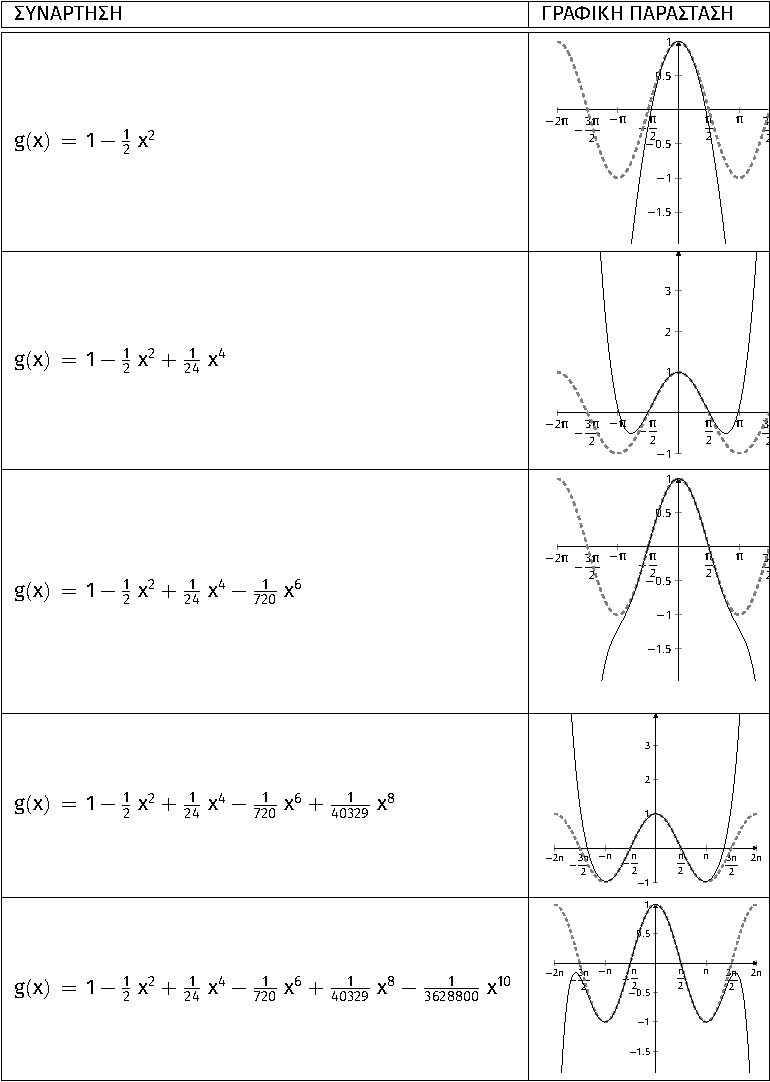
\includegraphics[width=0.99\textwidth]{tikzpic1.pdf}
%	\caption{Προσέγγιση της συνάρτησης $flate(x)=συν x$ μέσω πολυονύμων.}
%\end{figure}

\section*{Ασκήσεις}
\subsection*{Ορισμός-Ισότητα πολυωνύμων\hrule}
\begin{enumerate}[labelsep=20pt,label=\textbf{\arabic*.}]
	\item Να προσδιορίσετε τους πραγματικούς αριθμούς $α,β$, ώστε για κάθε \\${x\in \mathbb{R}-\{-1,1\}}$ να ισχύει:
	\[\dfrac{x+2}{(x-1)(x+1)}=\dfrac{α}{x-1}+\dfrac{β}{x+1} \]
	\solution{$α=\dfrac{3}{2}$, $β=1\dfrac{1}{2}$}
	\item Δίνεται το πολυώνυμο \[P(x)=(α^2-1)x^3+(|α|-1)x^2+α^3-1\]
	Να προσδιορίσετε τις τιμές του $α$, $α\in\mathbb{R}$, για τις οποίες $P(x):$\\
	\begin{multicols}{2}
		\begin{enumerate}[labelsep=5pt,label=\textbf{\greekalpha*.}]
			\item Είναι το μηδενικό πολυώνυμο\columnbreak
			\item Έχει βαθμό μηδέν.
		\end{enumerate}
	\end{multicols}
	\solution {α. $α=1$, β. $α= -1$}
	\item Να βρείτε το πολυώνυμο $P(x)$ για το οποίο ισχύει:
	\[(2x+5)\cdot P(x)=6x^3+x^2-33x+5\], για κάθε $x\in \mathbb{R}$ 
	\solution{$P(x)=3x^2-7x+1$}
	\item Δίνεται το πολυώνυμο:
	\[P(x)=(λ^2-4)x^4+x^3-5x^2+6x+4λ+6\]
	Αν το πολυώνυμο έχει ρίζα το 1, τότε να βρείτε το βαθμό του καθώς και την αριθμητική τιμή του για $x=2$.
	\solution{$λ=-2$, $P(x)=x^3-5x^2+6x-2$, $P(2)=-2$}
\end{enumerate}
\subsection*{Διαίρεση πολυωνύμων\hrule}
\begin{enumerate}[labelsep=20pt,label=\textbf{\arabic*.},resume]
	\item Να βρείτε το πολυώνυμο $P(x)$ το οποίο, όταν διαιρεθεί με το $x^2+1$, δίνει πηλίκο $2x-1$ και υπόλοιπο x+2.\solution{$P(x)=2x^3-x^2+3x+1$}
	\item Για το πολυώνυμο $P(x)$ ισχύουν οι σχέσεις $P(1)=0$ και $P(0)=1$. Να υπολογίσετε το υπόλοιπο της διαίρεσης $P(x):(x^2-x)$. \solution{$υ(x)-x+1$}
	\item Για το πολυώνυμο $P(x)$ ισχύουν οι σχέσεις:\[P(1)=3 \mbox{ και } P(2)=4\]
		\begin{enumerate}[labelsep=10pt,label=\textbf{\greekalpha*.}]
			\item Να βρείτε το υπόλοιπο της διαίρεσης του $P(x)$ με το $x^2-3x+2$.
			\item Αν επιπλέον είναι γνωστό ότι το $P(x)$ είναι τρίτου βαθμού και ισχύουν οι σχέσεις:
			\[P(0)=8 \mbox{ και } P(3)=17\]
				\begin{enumerate}[label=\textbf{\roman*.}]
					\item Να βρείτε το πηλίκο της διαίρεσης $P(x):(x^2-3x+2)$ καθώς και το πολυώνυμο $P(x)$.
					\item Να λύσετε την εξίσωση $P(ημx)=ημx+2$.
				\end{enumerate}
			\item Δίνεται το πολυώνυμο $P(x)=(x-1)^{2018}+αx+β$ για το οποίο είναι γνωστό ότι το υπόλοιπο της διαίρεσης $P(x):(x^2-2x))$ είναι το $x+2$.
			\begin{enumerate}
				\item Να βρείτε τους $α,β\in\mathbb{R}$.
				\item Να αποδείξετε ότι $P(x)>0$, για κάθε $x\in \mathbb{R}$.
			\end{enumerate}
		\end{enumerate}
\end{enumerate} 
				\solution{%
					\begin{minipage}[t]{1\linewidth}
					\begin{enumerate}[labelsep=10pt,label=\textbf{\greekalpha*.}]
						\item $υ(x)=x+2$
						\item 
						\begin{enumerate}[label=\textbf{\greekalpha*.}]
							\item $P(x)=x^3-6x+8$ 
							\item $x=2κπ+\dfrac{π}{2}\mbox{, }κ\in \mathbb{Z} $
						\end{enumerate}
					\end{enumerate}	
					\end{minipage}
					}
\subsection*{Θεωρήματα\hrule}
\begin{enumerate}[label=\textbf{\arabic*.},resume]
	\item Με χρήση του σχήματος Horner, να αποδείξετε ότι το πολυώνυμο 
		\begin{enumerate}[labelsep=20pt,label=\textbf{\greekalpha*.}]
			\item $P(x)=2x^4-6x^3+5x^2-3x+2$ έχει παράγοντα $(x-1)(x-2)$.
			\item $P(x)=x^4-5x^3+9x^2-8x+4$ έχει παράγοντα $(x-2)^2$.
		\end{enumerate}
		\solution{\begin{minipage}[t]{1\linewidth}		\begin{enumerate}[label=\textbf{\greekalpha*.}]
				\item $P(x)=(x-1)(x-2)(2x^2+1)$
				\item $P(x)=(x-2)^2(x^2-x+1)$
			\end{enumerate}\end{minipage}}
		\item Να αποδείξετε ότι αν το πολυώνυμο $P(x)$ έχει παράγοντα το $x-5$, τότε το πολυώνυμο $P(2x-3)$ έχει παράγοντα $x-4$.
		\item Το πολυώνυμο $P(x)$ είναι γνωστό ότι $P(1)=2$ και $P(3)-1$. Να βρείτε το υπόλοιπο της διαίρεσης του $P(x)$ με το $(x-1)(x-3)$.\solution{$υ(x)=-\dfrac{3}{2}x+\dfrac{7}{2}$}
		\item Αν για το πολυώνυμο $P(x)$ ισχύει: \[2P(x)+P(2-x)=-x^2-1 \mbox{, για κάθε } x\in\mathbb{R}\] τότε:
		\begin{enumerate}[label=\textbf{\greekalpha*.}]
			\item Να βρείτε τις τιμές $P(0)$ και $P(2)$.
			\item Να βρείτε το υπόλοιπο της διαίρεσης του $P(x)$ με το $x^2-2x$.
		\end{enumerate}
			\solution{\begin{minipage}[t]{1\linewidth}		\begin{enumerate}[label=\textbf{\greekalpha*.}]
						\item $P(0)=1$ και $P(2)=-3$
						\item $υ(x)=-2x+1$
					\end{enumerate}\end{minipage}}
\item Δίνεται το πολυώνυμο \[P(x)=x^3-2x^2+αx+β\]
Να βρέιτε τις τιμές των $α,β\in \mathbb{R}$ σε κάθε μία από τις παρακάτω περιπτώσεις:
\begin{enumerate}[label=\textbf{\greekalpha*.}]
	\item Αν το $P(x)$ έχει παράγοντα το $x-2$ και το υπόλοιπο της διαίρεσης $P(x):(x-1)$ είναι ίσο με $3$.
	\item Αν το $P(x)$ έχει παράγοντα το $x+2$ και το υπόλοιπο της διαίρεσης $P(x):(x+1)$ είναι ίσο με $6$.
	\item Αν τα υπόπολοιπα των διαιρέσεων  $P(x):(x+1)$ και $P(x):(x-2)$ είναι $-1$ και $4$ αντίστοιχα..
	\item Αν η αριθμητική τιμή του $P(x)$ για $x=1$ είναι ίση με $5$ και το $x-2$ είναι παράγοντας του $P(x)$.
	\item Αν το $P(x)$ έχει παράγοντα το $x^2-x-2$.
\end{enumerate}
\solution{\begin{minipage}[t]{1\linewidth}		\begin{enumerate}[label=\textbf{\greekalpha*.}]
			\item $α=-4, β=8$ 
			\item $α=-7, β=2$
			\item $α=\dfrac{2}{3}, β=\dfrac{8}{3}$
			\item $α=-6, β=12$
			\item $α=-1, β=2$
		\end{enumerate}\end{minipage}}
\end{enumerate}

\subsection*{Εξισώσεις- Ανισώσεις \hrule}

\begin{enumerate}[label=\textbf{\arabic*.},resume]
\item Να λύσετε τις εξισώσεις:
\begin{enumerate}[label=\textbf{\greekalpha*.}]
	\item $x^3+2x^2+3x+6=0$
	\item $x^3-7x^2+14x-8=0$
	\item $x^8-15x^4-16=0$
	\item $(x^2-2x-5)^2-2(x^2-2x)+2=0$
\end{enumerate}
\solution{\begin{minipage}[t]{1\linewidth}		\begin{enumerate}[label=\textbf{\greekalpha*.}]
			\item $-2$ 
			\item $1,2,4$
			\item $-2,2$
			\item $1-\sqrt{10}, 1+\sqrt{10},-1,3$
			\item $α=-1, β=2$
		\end{enumerate}\end{minipage}}
		\item Να λύσετε τις εξισώσεις:
		\begin{enumerate}[label=\textbf{\greekalpha*.}]
			\item $2x^4-5x^3+5x-2=0$
			\item $2x^4+5x^3-5x-2=0$
			\item $\dfrac{1}{3}x^3+\dfrac{7}{6}x^2+\dfrac{7}{6}x+\dfrac{1}{3}=0$
			\item $6x^4-5x^3-15x^2+4=0$
		\end{enumerate}
		\solution{\begin{minipage}[t]{1\linewidth}		\begin{enumerate}[label=\textbf{\greekalpha*.}]
					\item $1,-1,2,\frac{1}{2}$ 
					\item $1,-1,-2,-\frac{1}{2}$ 
					\item $-1,-2,-\frac{1}{2}$
					\item $-1,2,-\dfrac{2}{3},\dfrac{1}{2}$
				\end{enumerate}\end{minipage}}
		
		\item Να βρείτε το πρόσημο του γινομένου:
			\[P(x)=(x-2)(x^2-3x-4)(x^2+6x+9)(x^2-x+2)\]
			\solution{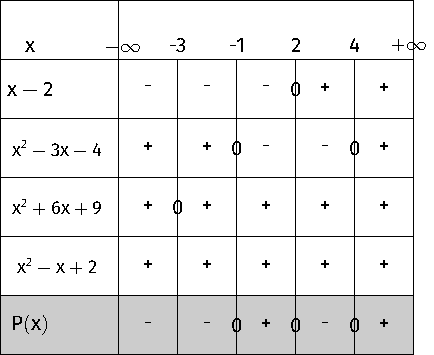
\includegraphics[valign=t]{15ASKpinakaki.pdf}}	
		\item Να λύσετε την ανίσωση \[x^4-3x^3-15x^2+19x+30\leq0\]
			\solution{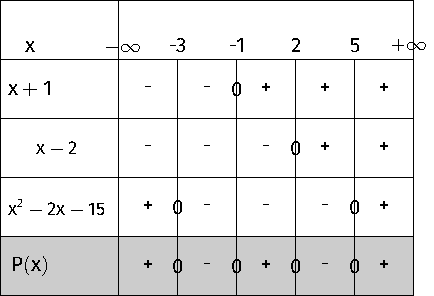
\includegraphics[valign=t]{16ASKpinakaki.pdf}
			\[	x\in[-3,-1]\cup[2,5]\]}
		\item Να λύσετε την ανίσωση $x^5-3x^4-6x^2+8 \geq0$ \solution{Θέτουμε $ω=x^2$. Τότε $x\in (-\infty,-2]\cup[-1,1]\cup[2,+\infty)$]}
		\item Να λύσετε την εξίσωση \[(x^2+2x-2)^3-(2x^2+4x-6)^2-23x^2-46x+68=0\]\solution{Θέτουμε $y=x^2+2x-2$. Τελικά οι ρίζες :$-4,-3,-1,1,2$}
		\item Δίνεται η συνάρτηση:\[f(x)=x^3+4x^2-7x-10\]Να βρείτε:
				\begin{enumerate}[label=\textbf{\greekalpha*.}]
				\item τα σημεία τομής της $C_f$ με τον άξονα $x'x$,
				\item τα διαστήματα στα οποία η $C_f$ βρίσκεται πάνω από τον άξονα $x'x$.
				\end{enumerate}\solution{\begin{enumerate}[label=\textbf{\greekalpha*.}]
					\item $A(-1,0)$, $Β(2,0)$, $Γ(-5,0)$
					\item $x\in(-5,-1)\cup(2,+\infty)$
				\end{enumerate}}
		\item Δίνεται το πολυώνυμο:\[P(x)=3x^3-14x^2+αx+β\]
		Η διαίρεση του $P(x)$ με το $x^2-4x-2$ αφήνει υπόλοιπο $(β-8)x+14-α$.
		\begin{enumerate}[label=\textbf{\greekalpha*.}]
			\item Να αποδείξετε ότι $α=6$ και $β=12$
			\item Να λύσετε την ανίσωση $P(x)\leq 4x+8$.\solution{$x\in\left(-\infty,2-\sqrt{6}\right)\cup\left[\dfrac{2}{3},2+\sqrt{6}\right]$}
		\end{enumerate}
		\item Έστω $P(x)$ 3ου Βαθμού το οποίο διαιρείται με το πολυώνυμο $x^2+2x$ και είναι τέτοιο, ώστε $P(1)=0$ και $P(2)=8$. \begin{enumerate}[label=\textbf{\greekalpha*.}]
			\item Να αποδείξετε ότι $P(x)x^3+x^2-2x$.
			\item Να λύσετε την εξίσωση $P(x)=8$.
			\item Να λύσετε την ανίσωση $P(x)>2$.
		\end{enumerate}\solution{
		\begin{enumerate}[label=\textbf{\greekalpha*.}]
		\item $α=1$, $β=-1$.
		\item $x=2$.
		\item $x\in \left(-\sqrt{2},-1\right)\cup\left(\sqrt{2},+\infty\right)$
		\end{enumerate}
		}%ΠΑΠΑΔΑΚΗΣ 17104
		\end{enumerate}
		
		
		
		\subsection*{Συνδιαστικές με συναρτήσεις \hrule}
		\begin{enumerate}[label=\textbf{\arabic*.},resume]
		\item \begin{minipage}[t]{0.5\textwidth}Στο διπλανό σχήμα δίνεται τμήμα της γραφικής παράστασης της συνάρτησης $f(x)=\dfrac{1}{4}x^3+γx+δ$ όπου $x\in\mathbb{R}$ και $γ,δ$ πραγματικές σταθερές.\end{minipage}
		\begin{minipage}[t]{0.5\textwidth}\centering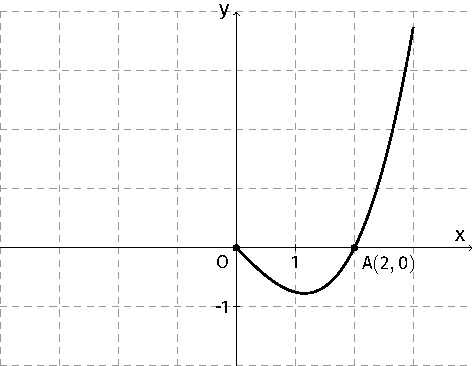
\includegraphics[scale=0.5,valign=t]{22ASKpinakaki.pdf}\end{minipage}
		\begin{enumerate}[label=\textbf{\greekalpha*.}]
			\item Με βάση τη γραφική παράσταση να αποδείξετε ότι $γ=-1$, $δ=0$.
			\item Θεωρώντας δεδομένο ότι $f(x)=\dfrac{1}{4}x^3-x$
				\begin{enumerate}
					\item Να αποδείξετε ότι: \\ $f(-x)=-f(x)$ για κάθε $x\in \mathbb{R}$
					\item Να μεταφέρετε στην κόλλα σας το σχήμα και να συμπληρώσετε τη γραφική παράσταση της $f$ για $x<0$.
					\item Να επαληθεύσετε ότι $f(1)=-\dfrac{3}{4}$ και στη συνέχεια να λύσετε τις εξισώσεις: \\
					$f(x)=-\dfrac{3}{4}$ και $f(x)\dfrac{3}{4}$
				\end{enumerate}
		\end{enumerate}
			\solution{\begin{enumerate}[label=\textbf{\greekalpha*.}]
					\item $f(0)=0$, $f(2)=0$
					\item 
					\begin{enumerate}[label=\textbf{\roman*.}]
						\item 
						\item 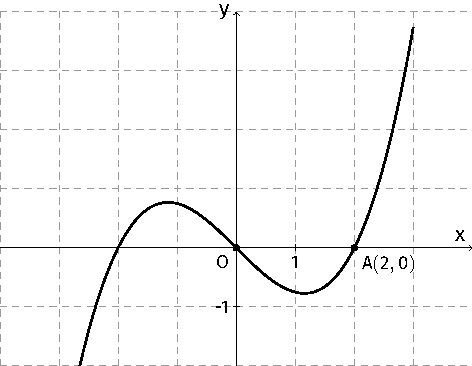
\includegraphics[scale=0.5,valign=t]{22bASKpinakaki.pdf}
						\item $-1$, $\dfrac{1-\sqrt{13}}{2}$,  $\dfrac{1+\sqrt{13}}{2}$
					\end{enumerate}\end{enumerate}
				}
		\item\begin{minipage}[t]{0.5\textwidth} Στο διπλανό σχήμα φαίνονται η γραφική παράσταση της συνάρτησης ${f(x)=-x^3-x^2}$ και η ευθεία που διέρχεται από τα σημεία $Α(0,1)$ και $Β(1,-2)$.
		\begin{enumerate}[label=\textbf{\greekalpha*.}]
			\item Να βρείτε την εξίσωση της ευθείας
			\item Αν η ευθεία έχει εξίσωση $y=-3x+1$ να βρείτε τις συντεταγμένες των κοινών σημείων της ευθείας με τη γραφική παράσταση της $f$
			\item Να λύσετε την ανίσωση \[-x^3-x^2<-3x+1\]
		\end{enumerate}\end{minipage}
		\begin{minipage}[t]{0.5\textwidth}\centering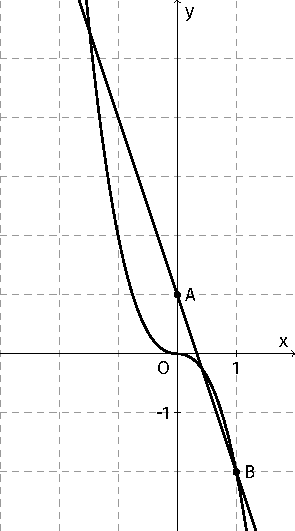
\includegraphics[scale=0.8,valign=t]{23ASKpinakaki.pdf}\end{minipage}
		\solution{
		\begin{enumerate}[label=\textbf{\greekalpha*.}]
			\item $y=-3x+1$
			\item $B(1,2)$,\\$Γ\left(-1+\sqrt{2}, 4-3\sqrt{2}\right)$, \\${Δ(-1-\sqrt{2},4+3\sqrt{2})}$
			\item $x\in \left(-1-\sqrt{2},-1+\sqrt{2}\right)\cup(1,+\infty)$
		\end{enumerate}
		}
\end{enumerate}



\subsection*{Εξισώσεις-Ανισώσεις που ανάγονται σε πολυωνυμικές \hrule}
\begin{enumerate}[label=\textbf{\arabic*.},resume]
				\item Να λυθεί η εξίσωση %Παπαδάκης σελ 331
				 \[\dfrac{1}{x+2}-\dfrac{3x-10}{x^2-4}=2x-\dfrac{x-3}{x-2}\]
				\solution{$x=-1$, $x=-\dfrac{1}{2}$}
				\item Να λυθεί η εξίσωση %Μιχαηλίδης σελ 613
				\[\dfrac{3x+11}{x^2-x-20}+2=\dfrac{2x-2}{x+4}\]
				\solution{$x=3$}
				\item Να λυθεί η εξίσωση \[(x-1)^2+\dfrac{1}{x^2-2x}=3\]
				\solution{Θέτουμε $ω=x^2-2x$ οπότε $x=1+\sqrt{2}$, $x=1-\sqrt{2}$}
				\item Να λυθεί η ανίσωση \[\dfrac{(x+2)(x^2-9)}{-x^2-2x+3}\geq 0\]
				\solution{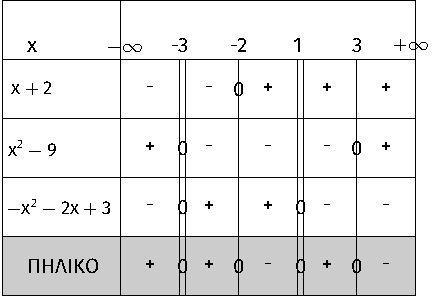
\includegraphics[scale=0.8,valign=t]{27ASKpinakaki.pdf} \[x\in(-\infty,-3)\cup(-3,-2]\cup(1,3]\]}
				\item Nα λυθεί η ανίσωση \[\dfrac{x^3+6x-5}{x^2-9}+\dfrac{3x}{x+3}+\dfrac{5}{x-3}+2\geq 0\]\solution{$x\in[-4,-3)\cup [-2,1]\cup(3,+\infty)$}
				\item Να λυθεί εξίσωση \[\sqrt{x+1}+1=x\]\solution{$x=3$}
				\item Να λυθεί εξίσωση \[\sqrt{2x+3}-\sqrt{x+1}=1\]\solution{$x=3$, $x=1$}
				\item Να λυθεί εξίσωση \[\sqrt{(x-1)^3}+\sqrt{4x-4}-5x+13=0\]\solution{Θέτουμε $ω=\sqrt{x-1}$, οπότε $x=5$, $x=17$}
\end{enumerate}

\subsection*{Επαναληπτικές - Θέματα εξετάσεων \hrule}
\begin{enumerate}[label=\textbf{\arabic*.},resume]
%ΠΑΠΑΔΑΚΗΣ 19.3
\item Δίνεται πολυώνυμο:\[P(x)=x^4-x^3+κx^2+x+λ \mbox{ , με } κ,λ\in \mathbb{R}\] 
\begin{enumerate}[label=\textbf{\greekalpha*.}]
	\item Να βρείτε τις τιμές των $κ, λ\in\mathbb{R}$ όταν το πολυώνυμο $P(x)$ έχει ρίζα το $1$ και παράγοντα $x+2$.
	\item  Για $κ=-7$ και $λ=6$ να λύσετε την εξίσωση $P(x)=0$.
	\item Για $κ=-7$ και $λ=6$ να λύσετε την ανίσωση: \[\dfrac{P(x)}{x-5}\geq 0\]
\end{enumerate}
\solution{
	\begin{enumerate}[label=\textbf{\greekalpha*.}]
	\item $κ=-7$, $λ=6$
	\item $x=1$ ή $x=-1$ ή $x=-2$ ή $x=3$
	\item $x\in [-2,-1]\cup[1,3]\cup(5,+\infty)$
	\end{enumerate}
}
%ΠΑΠΑΔΑΚΗΣ 19.8
\item Αν το πολυώνυμο
	\[P(x)=(λ^2-4)x^4+\dfrac{λ^2-λ-2}{4}x^3+3x^2+2λx-λ\]
	είναι 3ου βαθμού.
		\begin{enumerate}[label=\textbf{\greekalpha*.}]
			\item Να αποδείξετε ότι $λ=-2$.
			\item Να λύσετε την ανίσωση $P(x)\leq 14$.
			\item Αν $π(x)$ είναι το πηλίκο και $υ(x)$ είναι το υπόλοιπο της διαίρεσης $P(x):(x^2-1)$, να λύσετε την εξίσωση $\sqrt{π(x)}=υ(x)$.
		\end{enumerate}
		\solution{
			\begin{enumerate}[label=\textbf{\greekalpha*.}]
				\item $λ^2-4=0$ και $\dfrac{λ^2-λ-2}{4}\neq 0$
				\item $x\in(-\infty,-3]\cup[-2,2]$
				\item $π(x)=x+3$ και $υ(x)=-3x+5$, οπότε $x=1$.
			\end{enumerate}
			}
\item Δίνεται το πολυώνυμο 
		\[P(x)=2x^4+x^3+αx^2+βx+2\]
		το οποίο έχει παράγοντα $x^2-2x+1$.
		\begin{enumerate}[label=\textbf{\greekalpha*.}]
			\item Να βρείτε τις τιμές των $α,β\in \mathbb{R}$
			\item Να λύσετε την εξίσωση $P(x)=0$
			\item Να λύσετε την εξίσωση:\[2\left(\dfrac{1}{1+εφ^2x}\right)^2+συν^3x+6ημ^2x+συνx-4=0\]
		\end{enumerate}
		\solution{
			\begin{enumerate}[label=\textbf{\greekalpha*.}]
					\item $α=-6$, $β=1$
					\item $x=1$ ή $x=-2$ ή $x=-\dfrac{1}{2}$
					\item $συνx=1$ ή $συνx=-\dfrac{1}{2}$ $\iff x=2κπ \mbox{ ή  } x=2κπ \pm \dfrac{2π}{3}$
			\end{enumerate}
				}
\end{enumerate}
\newpage
\setlength{\columnsep}{20pt}\setlength{\columnseprule}{1pt}
\begin{multicols*}{2}
\theendnotes
\end{multicols*}
\end{document}